\documentclass[12pt, a4paper]{article}

\usepackage{amsmath}
\usepackage{array}
\usepackage[portuguese]{babel}
\usepackage{chngpage}
\usepackage{float}
\usepackage[a4paper, margin=2cm]{geometry}
\usepackage{graphicx}
\usepackage{hyperref}
\usepackage{setspace}
\usepackage{xcolor}

\title{\Huge \textbf{Computação Gráfica \\ \Large Trabalho Prático -- Fase I}}
\date{2 de março 2025}
\author{Grupo \textbf{\color{red} TODO}}

\begin{document}

\begin{center}
    
\includegraphics[width=0.25\textwidth]{res/cover/EE-C.eps}
\end{center}

\chardef\_=`_
\onehalfspacing
\setlength{\parskip}{\baselineskip}
\setlength{\parindent}{0pt}
\def\arraystretch{1.5}

{\let\newpage\relax\maketitle}
\maketitle
\thispagestyle{empty}

\vspace*{\fill}

\begin{adjustwidth}{-2cm}{-2cm} % These values only need to be large enough to center the table
    \begin{center}
        \begin{tabular}{>{\centering}p{0.25\textwidth}
                        >{\centering}p{0.25\textwidth}
                        >{\centering}p{0.25\textwidth}
                        >{\centering\arraybackslash}p{0.25\textwidth}}
            
\includegraphics[width=3.5cm]{res/cover/A104437.png} &
            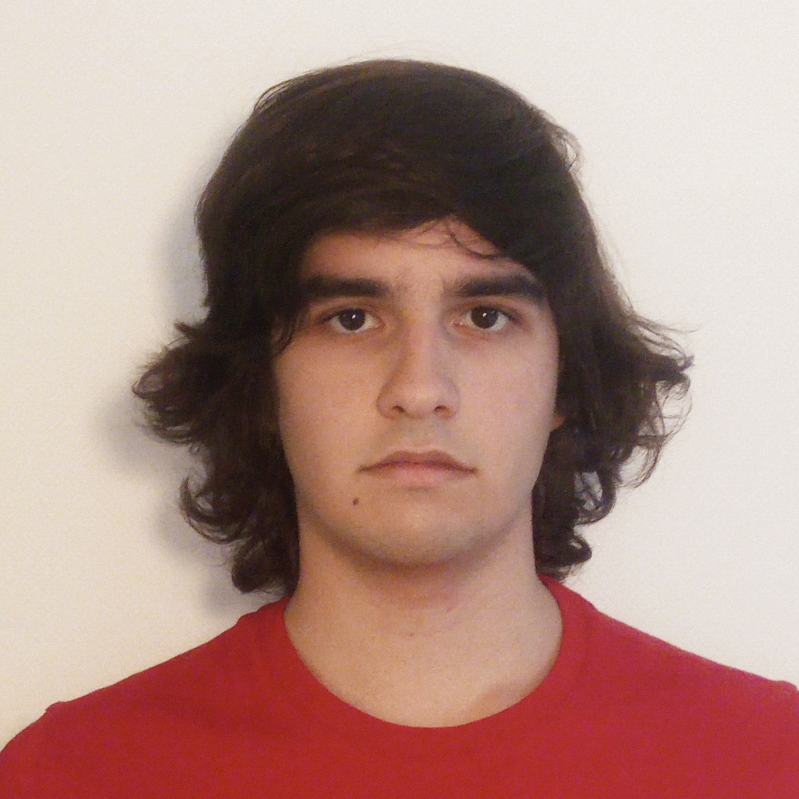
\includegraphics[width=3.5cm]{res/cover/A104348.png} &
            
\includegraphics[width=3.5cm]{res/cover/A90817.png} &
            
\includegraphics[width=3.5cm]{res/cover/A104179.png} \\

            Ana Oliveira & Humberto Gomes & Mariana Cristino & Sara Lopes \\
            A104437      & A104348        & A90817           & A104179
        \end{tabular}
    \end{center}
\end{adjustwidth}

\pagebreak

\begin{abstract}
    \textbf{\color{red} TODO - resumo}
\end{abstract}

\section{\emph{Generator}}

\subsection{Funcionamento do programa}

O programa \texttt{generator} é responsável por gerar modelos 3D de sólidos geométricos, ou seja,
ficheiros com os vértices e as faces triangulares destes sólidos. Nesta fase, o \texttt{generator}
deve ser capaz de gerar as seguintes figuras: planos, cubos, esferas e cones. Além de implementarmos
a geração destas figuras, como funcionalidade adicional, também desenvolvemos um gerador de
cilindros e de tori. As várias possibilidades de uso do comando \texttt{generator} são enumeradas
abaixo:

\begin{verbatim}
./generator plane    <length>      <divisions>                     <file>
./generator box      <length>      <grid>                          <file>
./generator sphere   <radius>      <slices>      <stacks>          <file>
./generator cone     <radius>      <height>      <slices> <stacks> <file>
./generator cylinder <radius>      <height>      <slices> <stacks> <file>
./generator torus    <majorRadius> <minorRadius> <slices> <stacks> <file>
\end{verbatim}

Internamente, o \texttt{generator} começa por interpretar os argumentos dados, saindo com a mensagem
acima em caso de erro. Caso contrário, gera, em memória, os conjuntos de vértices e de faces que
constituem o modelo 3D que, por fim, são escritos para um ficheiro no formato descrito abaixo.

\subsection{Formato \texttt{.3d}}

Decidimos que o formato de saída do \texttt{generator} seria o Wavefront OBJ \cite{wavefront-obj}.
O uso de um formato já existente apresentou diversas vantagens:

\begin{itemize}
    \item Foi possível desenvolver a \texttt{engine} e o \texttt{generator} em paralelo: os
        desenvolvedores do \texttt{generator} não precisavam de ter a \texttt{engine} funcional para
        testar o seu código, visto que já existem diversas ferramentas para visualizar os ficheiros
        OBJ exportados pelo \texttt{generator}.

    \item Foi possível, sem qualquer código adicional, apresentar na \texttt{engine} modelos 3D
        oriundos de ferramentas de modelação, muito mais complexos do que os gerados pelo
        \texttt{generator}.

    \item A forma de representação de faces triangulares neste formato é facilmente mapeável para
        \emph{index buffers} do OpenGL. Deste modo, não seriam necessárias alterações ao
        \texttt{generator} quando estes fossem implementados (algo que já foi feito nesta fase do
        trabalho).
\end{itemize}

O \emph{parser} desenvolvido para este formato suporta apenas o essencial para o funcionamento desta
primeira fase: posições de vértices e constituições de faces triangulares. O formato OBJ é textual,
e representar um vértice é tão simples como ter uma linha começada por um \texttt{v}, ao qual se
seguem as coordenadas do vértice separadas por espaços. O exemplo abaixo representa as coordenadas
$(0, 0.5, 1)$:

\begin{verbatim}
v 0 0.5 1
\end{verbatim}

Faces triangulares são representadas em linhas começadas por um \texttt{f}, ao qual se seguem os
índices dos três vértices da face. É de notar que a contagem dos índices começa em 1, e não em 0.
Por exemplo, para representar uma face triangular, formada pelo primeiro, segundo e terceiro
vértices do ficheiro, tem-se:

\begin{verbatim}
f 1 2 3
\end{verbatim}

\subsection{Cone}

Para gerar a nuvem de pontos do cone, é necessário ter em atenção dois vértices especiais, o centro
da sua base e o vértice do seu topo, com as coordenadas abaixo:

$$
P_0 = (0, 0, 0)
\hspace{1cm}
P_n = (0, H, 0)
\hspace{1cm}
\text{, onde $H$ representa a altura do cone}
$$

\begin{figure}[H]
    \centering
    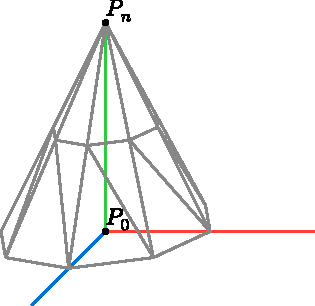
\includegraphics[width=0.35\textwidth]{res/figures/Cone1.pdf}
    \caption{Primeiro vértice ($P_0$) e último vértice ($P_n$) de um cone.}
\end{figure}

Os restantes vértices são todos obtidos do mesmo modo: para cada \emph{stack}, geram-se tantos
vértices quantos o número de \emph{slices}.

\begin{figure}[H]
    \centering
    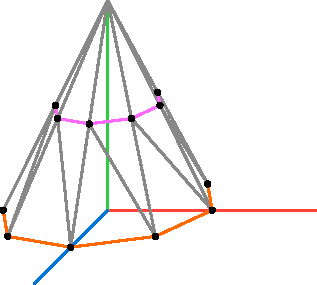
\includegraphics[width=0.4\textwidth]{res/figures/Cone2.pdf}
    \caption{
        Duas \emph{stacks} de um cone. Não são apresentados vértices ocultados pelas faces visíveis.
    }
\end{figure}

Para que as \emph{stacks} sejam equidistantes uma da outra, a distância entre \emph{stacks} será
o quociente entre a altura do cone e o número de \emph{stacks}. Por conseguinte, a coordenada $y$ da
$i$-ésima \emph{stack} será:

$$
y_i = \frac{H}{N_{stacks}} \times i
\hspace{1cm}
i \in \left \lbrace 0, 1, \ldots, N_{stacks} - 1 \right \rbrace
$$

Cada \emph{stack} no modelo será uma aproximação da secção transversal do cone por um plano
horizontal, ou seja uma circunferência. Na base do cone, o raio desta circunferência é o dado pelo
utilizador, $r$. Este raio tende para 0 à medida que se caminha para o vértice do topo do cone.
Logo, para a \emph{stack} $i$, o raio da circunferência a aproximar pode ser calculado por uma
interpolação linear:

$$
r_i = \frac{H - y_i}{H}\times r
\hspace{1cm}
i \in \left \lbrace 0, 1, \ldots, N_{stacks} - 1 \right \rbrace
$$

Dentro de cada $\emph{slice}$, as coordenadas $x$ e $z$ de cada ponto são determinadas de acordo
com a equação trigonométrica de uma circunferência:

$$
x = r_i \cos(\theta)
\hspace{1cm}
z = r_i \sin(\theta)
\hspace{1cm}
\theta \in \left [ 0, 2 \pi \right [
$$

Para se obterem tantos pontos quantas \emph{slices}, e para que estes estejam uniformemente
distribuídos pelo perímetro da circunferência, o ângulo $\theta$ é sempre incrementado em
$\frac{2 \pi}{N_{slices}}$ até o perímetro da circunferência ter sido coberto, dando origem à
seguinte equação de geração de pontos:

$$
x = r_i \cos \left ( \frac{2 \pi}{N_{slices}} \times j \right )
\hspace{1cm}
z = r_i \sin \left ( \frac{2 \pi}{N_{slices}} \times j \right )
\hspace{1cm}
j \in \left \lbrace 0, 1, \ldots, N_{slices} - 1 \right \rbrace
$$

Depois de estar criada a nuvem de pontos, constroem-se, em primeiro lugar, as faces triangulares da
base do cone. Para cada \emph{slice}, gera-se uma face, que tem  como vértices a origem ($P_0$), um
vértice da base ($P_1$), e o vértice da \emph{slice} seguinte ($P_2$), como mostra a figura abaixo:

\begin{figure}[H]
    \centering
    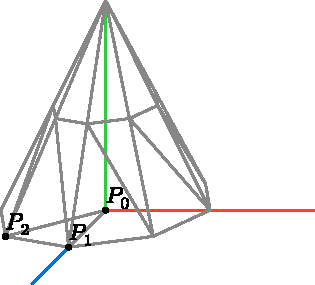
\includegraphics[width=0.4\textwidth]{res/figures/Cone3.pdf}
    \caption{
        \onehalfspacing
        Primeira iteração da construção das faces da base de um cone (com 8 \emph{slices} e 2
        \emph{stacks}).
    }
\end{figure}

Para que a normal desta face esteja voltada para fora do cone, ou seja, para baixo, os vértices do
triângulo são ordenados do seguinte modo, lembrando que esta ordem também se aplica aos restantes
vértices da base:

$$
T = (P_0, P_1, P_2)
$$

De seguida, constroem-se as faces laterais do cone, com exceção das da última \emph{stack} (a de
maior ordenada). É construído um quadrilátero (dois triângulos) por cada \emph{slice} na
\emph{stack}, utilizando um vértice da \emph{stack} ($P_1$), o seu adjacente seguinte na
\emph{stack} ($P_2$), e os dois pontos correspondentes a estes vértices na \emph{stack} seguinte
($P_9$ e $P_{10}$). A figura abaixo mostra os vértices utilizados na primeira iteração deste
processo:

\begin{figure}[H]
    \centering
    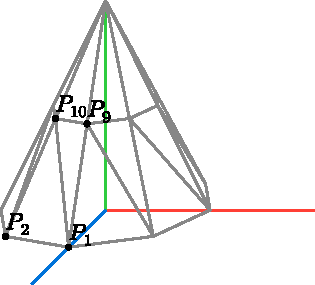
\includegraphics[width=0.4\textwidth]{res/figures/Cone4.pdf}
    \caption{
        \onehalfspacing
        Primeira iteração da construção das faces laterais de um cone (com 8 \emph{slices} e 2
        \emph{stacks}).
    }
\end{figure}

Para que os vetores normais destas faces apontem para fora do cone, utiliza-se a seguinte ordem para
os pontos dos triângulos, nesta e noutras iterações:

$$
T_1 = (P_1, P_9, P_{10})
\hspace{1cm}
T_2 = (P_1, P_{10}, P_2)
$$

Por último, constroem-se as faces da última \emph{stack}. Ao contrário do que acontece com as
restantes \emph{stacks}, já não se constroem quadriláteros, mas sim triângulos. Para cada
\emph{slice}, constrói-se um triângulo, formado pelo vértice do cone ($P_{17}$), por um vértice da
última \emph{stack} ($P_9$) e pelo vértice seguinte nessa \emph{stack} ($P_{10}$), como mostra a
figura abaixo:

\begin{figure}[H]
    \centering
    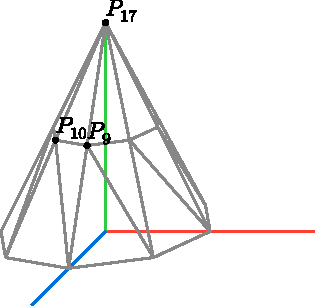
\includegraphics[width=0.4\textwidth]{res/figures/Cone5.pdf}
    \caption{
        \onehalfspacing
        Primeira iteração da construção das faces da última \emph{stack} de um cone (com 8
        \emph{slices} e 2 \emph{stacks}).
    }
\end{figure}

Para que estas faces sejam visíveis do exterior do cone, os seus vértices são ordenados do seguinte
modo:

$$
T = (P_9, P_{17}, P_{10})
$$

\section{\emph{Engine}}

\textbf{\color{red} TODO - \emph{engine}}

\section{Resultados obtidos}

\textbf{\color{red} TODO - resultados}

\section{Conclusão e Trabalho Futuro}

\textbf{\color{red} TODO - conclusão}

\begingroup
\section{Bibliografia}
\renewcommand{\section}[2]{}

\begin{thebibliography}{9}
    \bibitem{wavefront-obj}
        "Wavefront OBJ File Format Summary."{} FileFormat.Info. Accessed: Mar. 2, 2025. [Online.]
        Available: \url{https://www.fileformat.info/format/wavefrontobj/egff.htm}
\end{thebibliography}
\endgroup

\end{document}
